%!TEX root = main.tex
\section{Experiments and Results}\label{s:results}

% intro

%%%% 
% show that this approach is, in general, effective at discovering cellular automata.
\subsection{Bit consensus in n dimensions}

\CalloutFigure{f:002-fitness} shows the maximum fitness over time for 30 replicates each of three different experimental treatments: {\em logic}, {\em probabilistic}, and {\em adaptive}, each on a 1D cellular automata.  As shown here, fitness improves rapidly over time, eventually reaching a level of approximately 0.95 (recall that fitness is the correct fraction of 100 initial conditions).  \CalloutFigure{f:003-fitness} and \CalloutFigure{f:004-fitness} depict the results for 2- and 3-dimensions, respectively.  Taken together, these results indicate that this approach to discovering control strategies for cellular automata is quite effective.  Indeed, the results in 3-dimensions are the first known example of a bit-consensus controller for 3D CAs.

\begin{figure}
\centering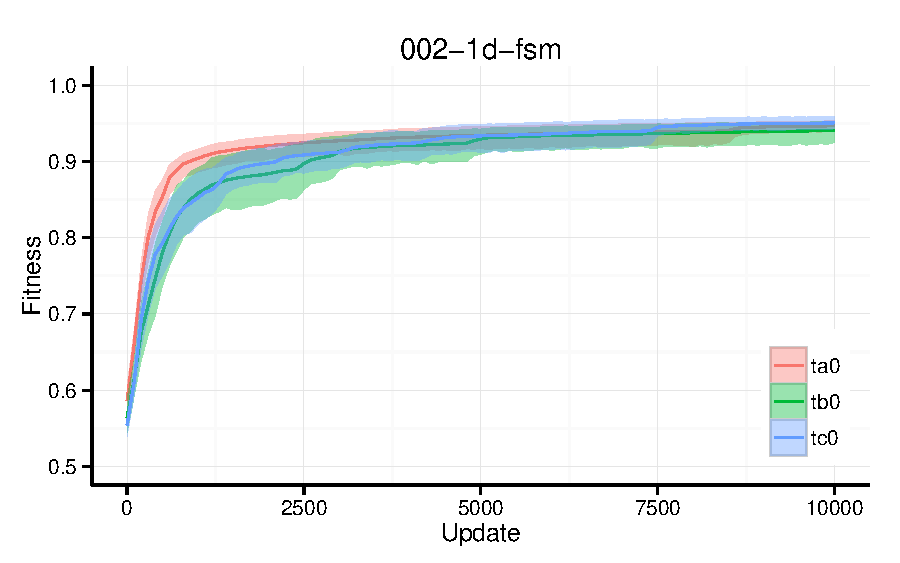
\includegraphics[width=\HalfPage]{x002-fitness}
\caption{}
\label{f:002-fitness}
\end{figure}

\begin{figure}
\centering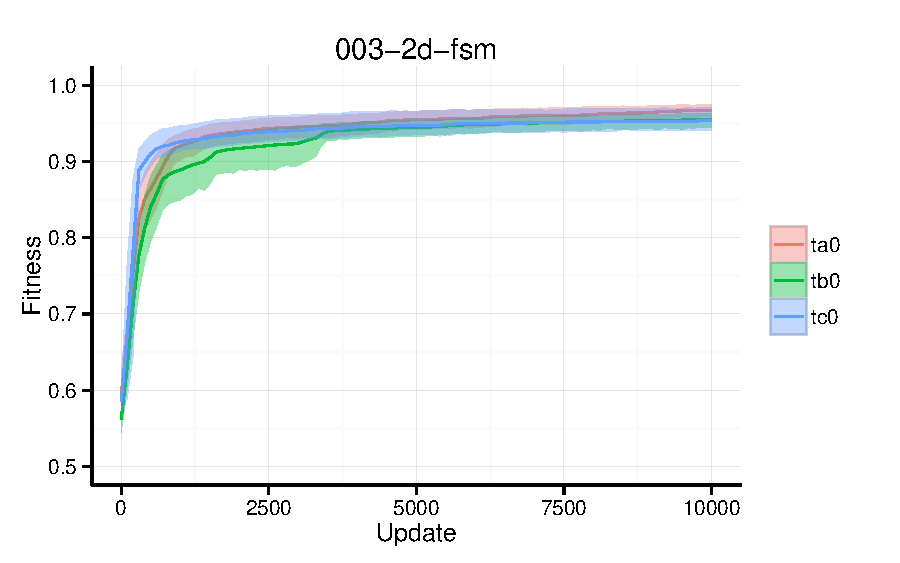
\includegraphics[width=\HalfPage]{x003-fitness}
\caption{}
\label{f:003-fitness}
\end{figure}

\begin{figure}
\centering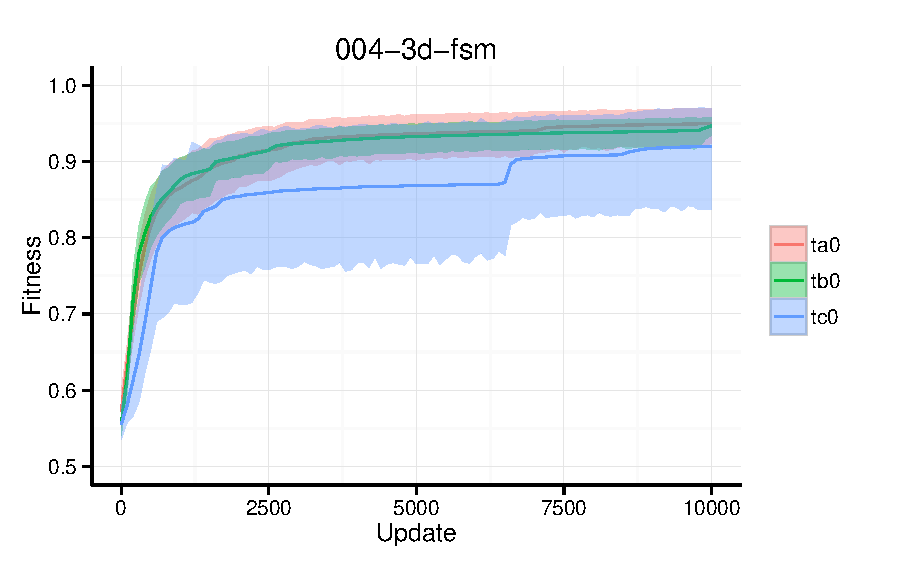
\includegraphics[width=\HalfPage]{x004-fitness}
\caption{}
\label{f:004-fitness}
\end{figure}

\CalloutFigure{f:002-detail} depicts the state of the cellular automata over time for the dominant (most fit) individual from the 1d CA.  This illustration shows how information from different regions of the state vector are used to produce coherent changes over time.
% + Mitchell

\begin{figure}
\centering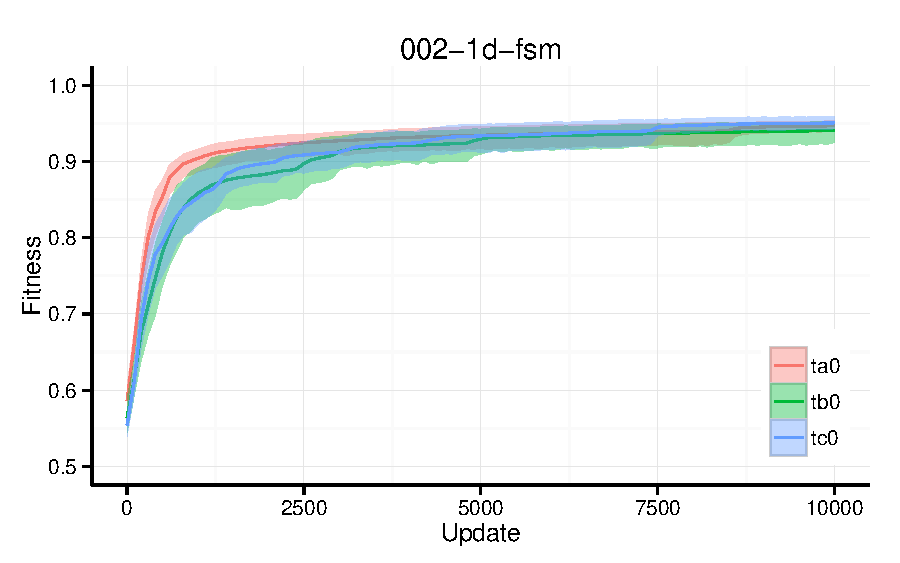
\includegraphics[width=\HalfPage]{x002-fitness}
\caption{}
\label{f:002-detail}
\end{figure}

\CalloutFigure{f:003-detail} depicts CA state in 2d; here we present a number of frames from a movie, the entirety of which can be found here: \url{?}.  Though somewhat more difficult to see in 2d, there are similarities apparent between the strategy shown in 1d and here, particularly in the ``wavefront'' style activations.

\begin{figure}
\centering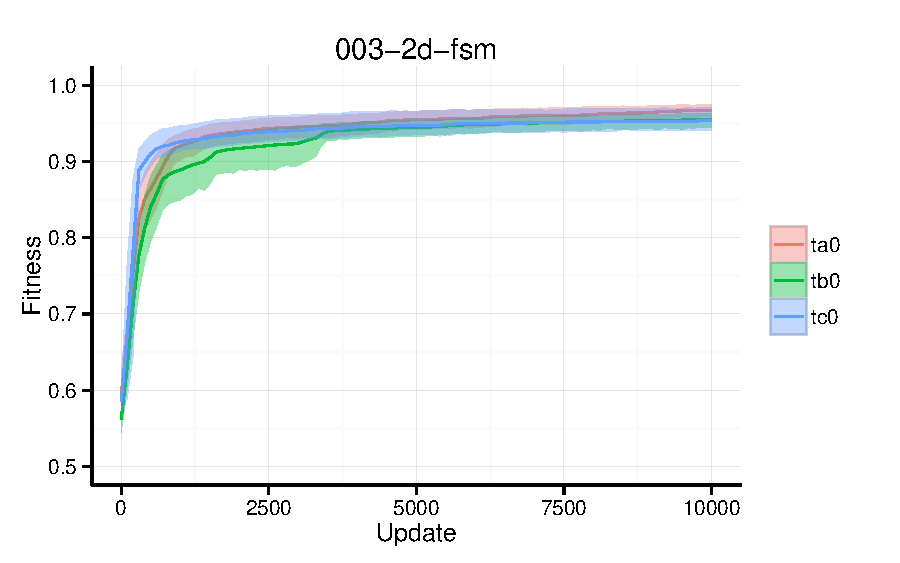
\includegraphics[width=\HalfPage]{x003-fitness}
\caption{}
\label{f:003-detail}
\end{figure}

Finally, \CalloutFigure{f::004-detail} depicts CA state in 3d; we again present a number of frames from a movie, which can be found here: \url{?}.

\begin{figure}
\centering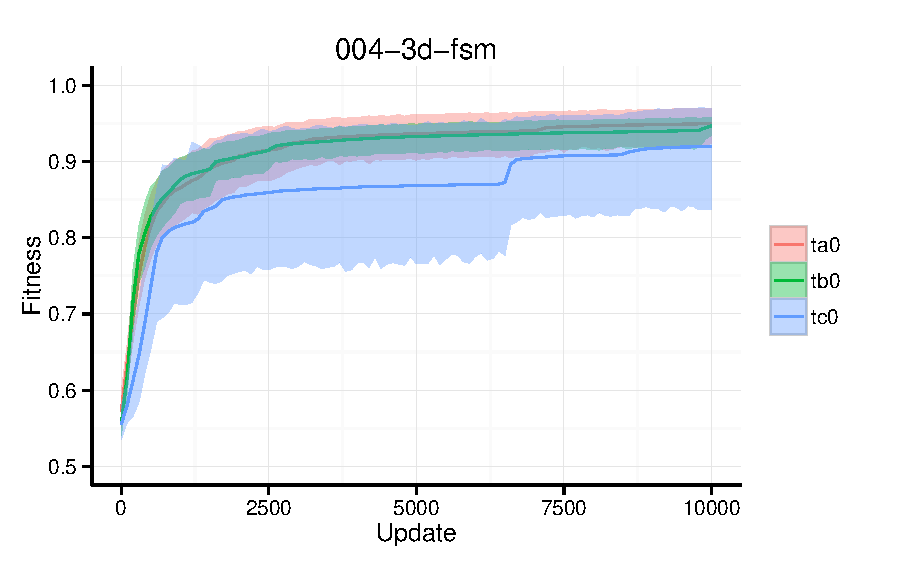
\includegraphics[width=\HalfPage]{x004-fitness}
\caption{}
\label{f:004-detail}
\end{figure}


%%%%
% show that the evolved solutions are, in fact, self-organizing, and that they have properties that are desirable in SO systems: scalable, resilient
\subsection{Self-organization}

We can test for self-organization as a property by manipulating the communication channel(s) between cells in the CA.  Specifically, if a given CA is self-organized, its performance {\em in the absence} of communication will be significantly less than if communication is allowed.  \CalloutFigure{f:selforg} depicts the unit function \dk{see manet paper} for self-organization on each of the dominant solutions from all treatments in 1-, 2-, and 3-dimensions.
% use 0; no information

\begin{figure}
\centering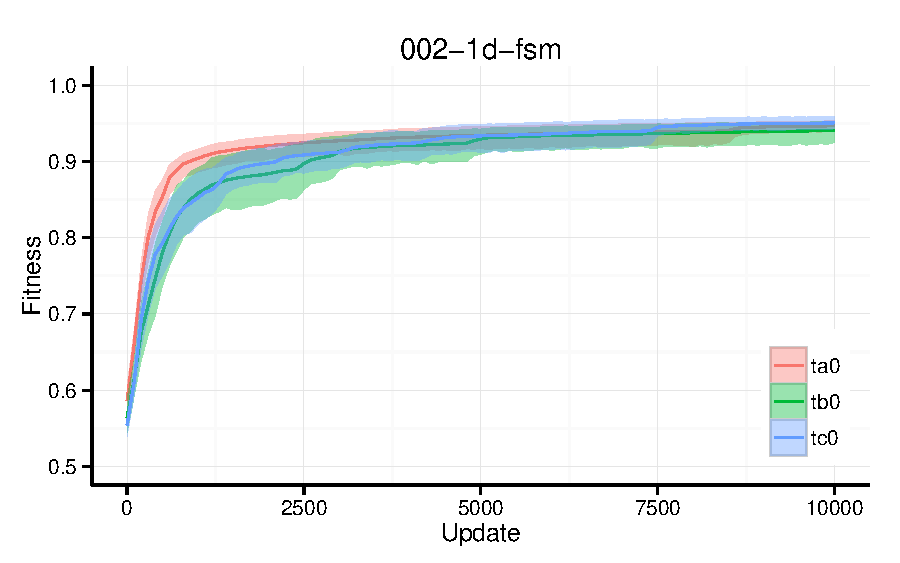
\includegraphics[width=\HalfPage]{x002-fitness}
\caption{}
\label{f:selforg}
\end{figure}

% scalability
A key desirable characteristic of self-organizing systems is that they scale to larger instances without code changes.  \CalloutFigure{f:scalability} depicts the scalability of dominant individuals from each of the different treatments over a range of different CA sizes.  As seen here, the evolved solutions are highly scalable, in some cases scaling multiple orders of magnitude above their evolved size with no decline in performance.

\begin{figure}
\centering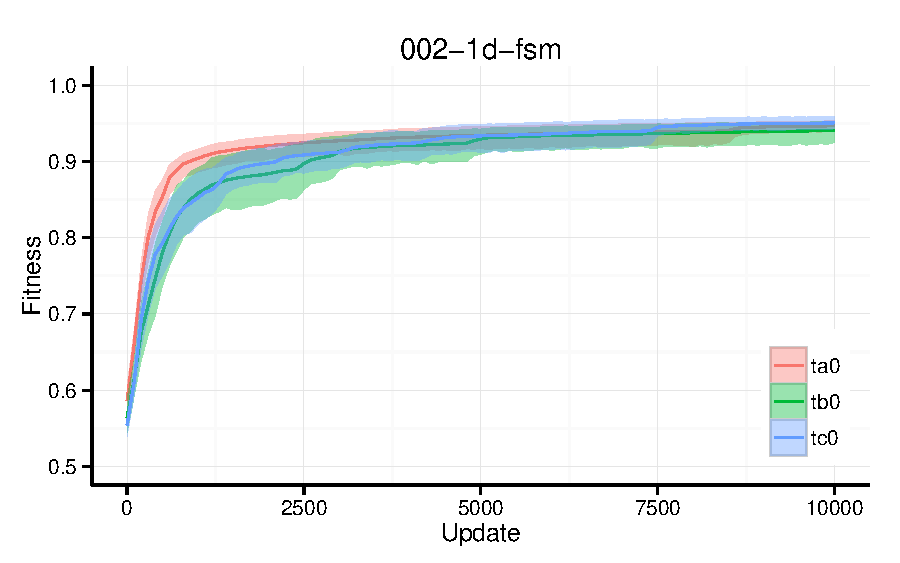
\includegraphics[width=\HalfPage]{x002-fitness}
\caption{}
\label{f:scalability}
\end{figure}

% resilience
A key characteristic of SASO systems is that they are resilient in the face of environmental disturbances.  Here, we can model such conditions by perturbing the state vector of a CA over time.  With a configurable probability, here we examine the effect of randomly changing the state vector at a single point in time {\em after} the CA has reached a stable solution.  Depending on the probability of noise, this should still result in the CA reaching the correct solution.  Results are shown in \CalloutFigure{f:resilience}
% use random; noise

\begin{figure}
\centering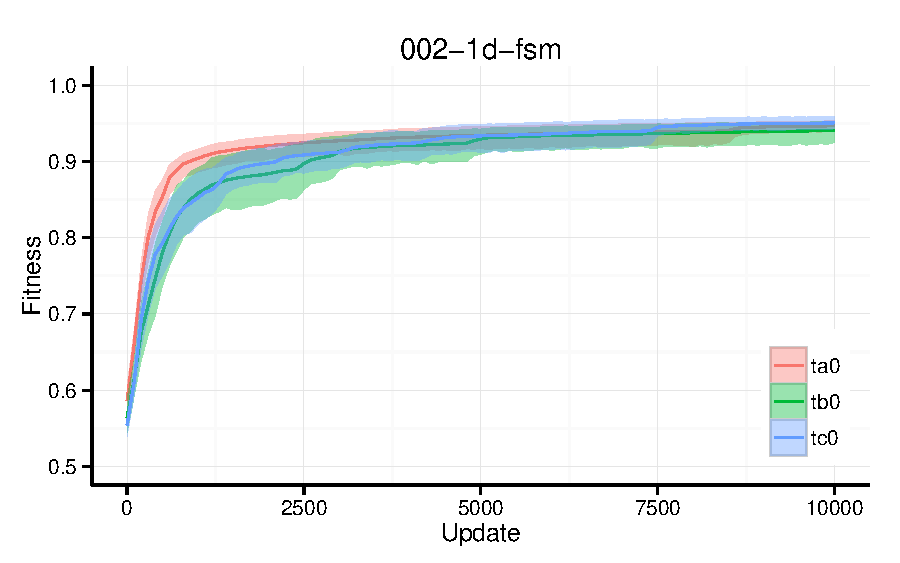
\includegraphics[width=\HalfPage]{x002-fitness}
\caption{}
\label{f:resilience}
\end{figure}

%%%%
% show that (some approaches) are also self-adaptive
\subsection{Self-adaptation}

1P: is self-adaptation being used?  if so, there's an endogenous RL signal that the state machine is generating.  what happens when that RL signal is external?

2P: performance when an external RL signal is available; this is more interesting than thought: it's a global signal, not individual to the cell; each cell must somehow detangle what it did w.r.t. global signal

3P: two ways to handle this: incorporate changing goals into fitness function (anticipated adaptation), or re-evolve to meet new goal (unanticipated adaptation).






%In this section, we present our experiments and results on using {\neat} to evolve neural network controllers for the nodes in a mobile ad hoc network.  When evaluating a given ANN, nodes in the simulation shared the same neural network structure (neurons, links), but had their own instance of the neural network -- It may be helpful to think of a MANET as a single homogeneous population of neural networks.  In all of the experiments presented below, we require that the network: (1) be connected at the time of fitness evaluation, and (2) that the centroid of the network less than 200m from the origin, otherwise the minimum possible fitness is assigned to that individual (note that it may still be selected for recombination, though this is unlikely).  These steps were optimizations to reduce computation time.


%%%%
%\subsection{Motivating Experiment}\label{s:baseline}
%Our first experiment investigated the evolution of neural networks that could solve the grid-coverage problem, and it provides the motivation for the following experiments.  Specifically, the fitness function used here was simply that shown in \CalloutEqn{e:grid-coverage}, which was evaluated after 10s of simulation time.
%
%\CalloutFigure{f:1-fixed-network} plots the mean normalized fitness of the dominant (most fit) individual per generation across 30 separate trials for both 8-node ($FF8$) and 16-node ($FF16$) networks.  The (very small) error bars in this and other figures are 95\% confidence intervals constructed via 200-fold bootstrapping.  We define {\em normalized fitness} as $f/f_{max}$, where $f_{max}$ is the maximum possible fitness achievable given the fitness function and network size.  In this treatment, fitness and normalized fitness are identical, although that is not the case in many of the following experiments.  In \CalloutFigure{f:1-fixed-network}, we see that the dominant individuals in 8-node networks reach their optimal fitness after approximately 40 generations, while 16-node networks averaged only $71.5\pm0.6$\% after 200 generations.
%%(We note that fitness calculation is slightly different [10s as opposed to here than in previous experiments, thus these results are not exactly the same as in \CalloutSection{s:results-complex}.)
% 
%\begin{figure}[htb]
%\centering\includegraphics[width=\HalfPage]{1-fixed-network}
%\caption{Normalized fitness of 8- and 16-node fixed-size networks using a fitness function that rewards only for grid-coverage.}
%\label{f:1-fixed-network}
%\end{figure}
%
%Upon examination of the evolved behaviors, the reason for the decline in fitness of 16-node networks became apparent: For both 8- and 16-node networks, the evolved strategies were primarily stochastic, and relied upon the continual movement of nodes throughout the environment.  One such behavior is depicted in \CalloutFigure{f:2-fixed-movement}, which shows the position and velocity vectors of each node in the 16-node network over 20s of simulation time.  In this figure, nodes start in an array along the $x-$axis, and generally move in a spiral pattern within the region bounded by the grid.  A movie of this behavior (and others described in the following sections) is available at: \url{http://www.cse.msu.edu/thinktank/manet}.  This behavior was also prevalent in the smaller 8-node networks.  The reason this strategy is effective is related to the size of the grid relative to the number of nodes in the network.  On average, if the grid is large relative to the size of the network, and nodes maintain some distance between each other while moving over the grid, nodes are likely to be in different cells at the time of fitness evaluation.  This strategy is less effective with larger MANETs because nodes are more likely to occupy the same cell.  Interestingly, this strategy is not unlike that exhibited in flocks of starlings~\cite{fernandez-juricic2004flock}, where individuals adjust their movements to maintain a ``safe'' distance amongst themselves.
%
%\begin{figure}[htb]
%\centering\includegraphics[width=\HalfPage]{2-fixed-movement}
%\caption{Sample velocity and position of a 16-node network following 20s of control ($FF16$ treatment).  Nodes start at $(x,0)$, and then move in a spiral for the remainder of the simulation.}
%\label{f:2-fixed-movement}
%\end{figure}
%
%However, from the perspective of engineering controllers for a MANET, these evolved behaviors are lacking in two significant ways: First, the evolved behaviors are {\em unstable}.  We expected to see behaviors where nodes would deterministically move to unique cells in the grid and stop moving.  Instead, the nodes moved continually in a spiral pattern, which would waste energy in a real network.  Second, these behaviors do not {\em scale}.  We hoped to evolve effective behaviors for networks of varying size.  However, we found that normalized fitness decreased as network size increased, a result which we verified on larger 32-node networks and both larger and smaller grids.  In all cases, the key factor was the number of nodes being controlled, which is known to be a challenge for multi-agent systems~\cite{panait2005cooperative}.  In the following experiments, we examine ways to improve network stability and scalability.
%
%
%%%%%
%\subsection{Stable Networks}\label{s:speed}
%Based on the behaviors observed in the previous experiment, we first explored ways to improve network stability.  The goal here was to discover networks whose nodes would move to and then settle in a location, instead of continuing to move throughout the environment.  Our first approach was to devise a fitness function that included a speed component, such that networks with nodes that were moving slowly at the time of fitness evaluation would have a higher fitness than a network whose nodes were moving quickly.  This fitness function, $SF(M)$, rewarded for a reduction in the average speed at which nodes in $M$ (the MANET) were moving, specifically:
%%
%\begin{equation}
%SF(M) = \frac{G(M,36)}{10\cdot\max(0.1, \overline{\mathrm{spd}(M)})}
%\label{e:sf}
%\end{equation}
%%
%where $G(M,36)$ is performance on the 36-cell grid-coverage problem, and $\overline{\mathrm{spd}(M)}$ is the average speed of all nodes in $M$ at the end of the simulation.  The other components of this fitness function, scaling by 10 and $\max(\cdot)$, were used to ensure that the resulting fitness score is in the range $[0..1]$.  This fitness function thus rewards MANETs that quickly move to, and settle, in a stable configuration.
%
%\CalloutFigure{f:3-slow-network} plots the mean normalized fitness of the dominant individual per generation over 30 trials on networks of 16 nodes.  Surprisingly, the mean normalized fitness of dominant individuals under this treatment is $55.3\pm1.2$\% after 200 generations, which is even worse than in the base $FF16$ case.  Upon examination of the evolved behaviors, however, we did indeed find that the networks exhibited the desired behavior, where nodes stabilized into a fixed position after reaching their target cells, although many nodes shared occupancy of cells.
%
%\begin{figure}[htb]
%\centering\includegraphics[width=\HalfPage]{3-slow-network}
%\caption{Normalized fitness for 16-node networks that are rewarded for reduced speed.}
%\label{f:3-slow-network}
%\end{figure}
%
%%Upon examination of the evolved behaviors, we did indeed find that the networks exhibited the desired behavior, where nodes stabilized into a fixed position after reaching their target cells.  An example of this behavior is shown in \CalloutFigure{f:4-slow-movement}, which shows the position and velocity of each node during 20s of simulation time.  Nodes again start in an array along the $x-$axis, and slowly move to different grid cells, although many nodes share cells.%  A video of this behavior is available at: \url{http://somewhere-else}.
%
%%\begin{figure}[htb]
%%\centering\includegraphics[width=\HalfPage]{4-slow-movement}
%%\caption{Velocity and position of 16 nodes in the network evolved under treatment $SF16$, which rewards for a reduction in the average speed of nodes at the end of the simulation.}
%%\label{f:4-slow-movement}
%%\end{figure}
%
%%%%%
%\subsection{Reducing Entropy}\label{s:redentropy}
%One key difference we noticed between this behavior and that shown in \CalloutFigure{f:2-fixed-movement} is that here the behavior of individual nodes was based on their starting location in the environment, and did not appear to be stochastic.  {\em Information entropy} is frequently used to characterize stochastic processes~\cite{shannon1948a-mathematical}.  To measure information entropy, $H(X)$, of a mobile network, we leverage the following definition:
%%
%\begin{equation}
%H(X) = -\sum_{i=1}^{n}p(x_{i})\log_{2}p(x_{i})
%\label{e:entropy}
%\end{equation}
%%
%where $X=\{x_{1}, \dots, x_{n}\}$ is the discrete random variable representing the states of the network, and $p(\cdot)$ is the probability mass function of $X$.  We define the states of $X$ based on the cells of the grid occupied by nodes in the network.  Specifically, each possible value of $X$ is a length-$k$ bitstring, where $k$ is the number of cells in the grid (36, in this study).  A ``1'' at position $i$ in this bitstring represents that cell $i$ is occupied by at least one node, while a ``0'' indicates that cell $i$ is not occupied.  The frequencies of these states during a simulation defines $p(\cdot)$.  Intuitively, a high value for information entropy represents a network that exhibits many states with low frequency, while a low value represents a network that exhibits few states with high frequency.  We assume that low information entropy is a desirable property of engineered systems.  For brevity, in the remainder of this paper we will refer to this calculation as the {\em entropy} of a network.
%
%\CalloutFigure{f:5-entropy} plots the mean entropy for the dominant individuals per generation over all 30 trials for two treatments: $FF16$, described in \CalloutSection{s:baseline}, whose fitness function did not include a velocity component; and $SF16$, described in this section, where a reward for reduced velocity was included as part of fitness.  As would be expected, here we see that entropy of the $SF16$ treatment is significantly lower than that of the $FF16$ treatment, indicating a more stable behaviors.
%
%\begin{figure}[htb]
%\centering\includegraphics[width=\HalfPage]{5-entropy}
%\caption{Entropy on 16-node networks under a treatment rewarding only for grid-coverage ($FF16$) and the grid-coverage plus reduced velocity ($SF16$).}
%\label{f:5-entropy}
%\end{figure}
%
%To further explore the relationship between entropy and behavior, we also devised a fitness function that rewarded explicitly for a reduction in entropy, with no consideration given to speed.  Though their performance on the grid-coverage problem was similar, the evolved behaviors were markedly different.  Specifically, when using a fitness function that rewarded for reduced entropy instead of average speed, nodes were likely to start by moving very slowly, but then would accelerate as the simulation progressed, eventually moving off the grid (data not shown).  For this reason, our subsequent experiments include speed-reduction, which implicitly reduces entropy, as a component of fitness.%, instead of an explicit reward for reduced entropy
%
%% -- In other words, while we consider low entropy to be a desirable characteristic, 
%%
%%while we consider low entropy to be a desirable characteristic, 
%%
%%our subsequent experiments include speed-reduction as a component of fitness instead of an explicit reward for reduced entropy.
%
%%\begin{figure}[htb]
%%\centering\includegraphics[width=\HalfPage]{6-entropy-movement}
%%\caption{Velocity and position of 16 nodes in a network evolved a treatment that rewarded for a reduced entropy explicitly; nodes did not stabilize into a fixed position, instead moving off the grid.}
%%\label{f:6-entropy-movement}
%%\end{figure}
%%
%%While we found that rewarding for reduced speed improved both stability and entropy of the evolved behaviors, we also noticed that these behaviors were {\em static}; that is, individual nodes no longer reacted to the presence (or absence) of neighboring nodes.
%
%%The second treatment, $EF8$, included entropy directly as part of the fitness function.  Specifically:
%%%
%%\begin{equation}
%%EF8(M) = G_{8}(M) + \frac{1}{\clip(H(M), 1, 10)}
%%\label{e:ef8}
%%\end{equation}
%%%
%%where $EF8(M)$ is fitness; $G_{8}(M)$ is again performance on the grid-coverage problem; and $H(M)$ is the entropy of the MANET calculated according to \CalloutEqn{e:entropy}, clipped to the range $[1.0, 10.0]$ to ensure that the contribution of entropy to fitness was of an equivalent range as performance on the grid-coverage problem.
%%
%%\CalloutFigure{f:sf8-ef8} contains plots of the results of these two treatments, again showing mean fitness, entropy, self-organization, and scalability of the dominants over 200 generations.  Here we see that the $EF8$ treatment out-performs the $SF8$ treatment, though their entropies are not statistically significantly different (Wilcoxon rank sum test, $p=0.45$).  We note that the difference in fitness is driven by the additional term in the fitness functions (average velocity and entropy, respectively) -- The performances of these treatments on the grid-coverage problem in isolation were not statistically significantly different ($p=0.516$, mean$=0.678$).  \dk{Because these treatments are essentially equivalent in their performance and entropy, we selected to further explore treatment $SF8$ based on the character of its behavior, which we found to be more stable than the behaviors produced by treatment $EF8$.  Specifically, rewarding for reduced velocity produced behaviors where nodes would quickly move to, and settle, in different cells.}  \dk{Entropy is important, but rewarding for a reduction in entropy isn't sufficient to evolve the kinds of behaviors that we'd like to see.}  We next explore ways to increase operational self-organization.
%%
%%%\begin{figure}
%%%\centering\includegraphics[width=\textwidth]{308-fneatab-components}
%%%\caption{Fitness and entropy on fixed-size networks of 8 nodes while rewarding for a decrease in velocity and entropy.}
%%%\label{f:sf8-ef8}
%%%\end{figure}
%
%
%%%%%
%\subsection{Reactive Networks}\label{s:selforg}
%Thus far, we have considered several approaches to the evolution of controllers and identified three main challenges.  The first, which we have addressed by rewarding for a reduction in average node speed, was that evolved behaviors tended to be stochastic.  Second, we found that when fitness includes a reward for stability, the evolved behaviors were not reactive.  Finally, we found that fitness decreased as the number of nodes in the network increased, identifying scalability as a concern as well.  To address these final two challenges, we investigated two new approaches that varied the number of nodes in the network during the course of the simulation.  Our hypothesis was that if the number of nodes in the simulation changed over time, then individual nodes would have to react to each other in order to achieve a high fitness, and that this would result in reactive and scalable behaviors.
%
%For these two approaches, we initialized each simulation with a MANET comprising only 2 nodes.  In the first treatment, $SV2$, we unconditionally added 2 nodes to the simulation environment every 5s, and ran the simulation for a total of 120s (48 total nodes at the end of the simulation; the grid remained unchanged at 36 cells), at which point fitness was calculated.  The second treatment, $SV2G$, was configured identically, except that nodes were added only if the existing network had a normalized fitness greater than 80\%.  This second treatment was inspired by the idea of ``building blocks'' in genetic algorithms.  In this case, the building block is a behavior for a smaller network.  In both cases, we used the fitness function shown in \CalloutEqn{e:sf}.  We note that for these treatments, the calculation of normalized fitness is done with respect to the number of nodes that would be present in the network assuming optimal control.
%
%\CalloutFigure{f:7-var2-fitness} plots the mean normalized fitness of the dominant individual per generation over 30 trials of each of these two treatments.  In general, fitnesses and evolved behaviors under these two treatments were poor.  In the $SV2$ treatment, where nodes were unconditionally added, a common behavior was for nodes to slowly move across the grid, relying on the addition of new (also slow-moving) nodes to achieve higher fitness.
%
%\begin{figure}[htb]
%\centering\includegraphics[width=\HalfPage]{7-var2-fitness}
%\caption{Normalized fitness for treatments where nodes are added to the simulation unconditionally ($SV2$), and conditionally based on the existing network reaching 80\% of its possible fitness ($SV2G$).}
%\label{f:7-var2-fitness}
%\end{figure}
%
%The poor performance of the $SV2G$ treatment is explained by the small number of nodes that were being controlled: In the best case overall, only 12 nodes (out of a possible 48) were controlled following 200 generations of evolution.  However, we did notice that the more successful behaviors appeared to depend on interaction among individuals, which we tested by turning communication off and re-evaluating the dominant evolved solutions.% (this was not the case in the $SV2$ treatment).  %\CalloutFigure{f:8-var2-movement} depicts one such reactive behavior, showing the position and velocity of each node during 20s of simulation time.  Here, 2 nodes start along the $x-$axis, and quickly move to and settle in different nearby cells, achieving greater than 80\% fitness and triggering the addition of more nodes.  Then, as additional nodes join the network, they adapt to each others' presence, and spread out along the $x-$ and $y-$axes to occupy different cells.  A video is available at: \url{http://a-different-place}.
%
%%\begin{figure}[htb]
%%\centering\includegraphics[width=\HalfPage]{8-var2-movement}
%%\caption{Velocity and positions of an example individual evolved under the $SV2G$ treatment.}
%%\label{f:8-var2-movement}
%%\end{figure}
%
%%\dk{add in a time-lapsed scatter plot where different nodes are colored differently, or rely on the movie?}
%
%This property, where individuals react to each other locally without regard to a global pattern, is an example of {\em self-organization}.  There are numerous definitions for self-organization.  For example, Haken~\cite{haken2006information} states that, ``A system is self-organizing if it acquires a spatial, temporal, or functional structure without specific interference from the outside.''  Another definition is provided by Camazine~\cite{camazine2003self}: ``Self-organization is a process in which pattern at the global level of a system emerges solely from numerous interactions among the lower-level components of the system.''  Likewise, numerous metrics have been proposed for how to measure self-organization~\cite{polani2003measuring, schmeck2010adaptivity, yamins2005towards}.  However, in the context of evolving a solution to the grid-coverage problem, what is needed is a way to ensure that the neural networks produced via evolution are communicating to solve the overall problem.  We thus define {\em operational self-organization}, $S_{op}(x)$, of a neural network $x$, as:
%%
%\begin{equation}
%S_{op}(x) =\frac{f(x)-f_{nc}(x)}{f(x)+f_{nc}(x)}
%\label{e:self-org}
%\end{equation}
%%
%where $f(x)$ is the fitness of the neural network $x$ with communication among agents enabled and $f_{nc}(x)$ is fitness with communication among agents disabled.  $S_{op}(x)$ has the interesting property that values greater than zero indicate the presence of self-organization (communication is beneficial), while values less than or equal to zero indicate the lack of self-organization (communication is harmful or neutral).
%
%We calculated operational self-organization for the dominant solutions from all of the treatments previously presented; results are shown in \CalloutFigure{f:9-selforg}.  Surprisingly, we see that the original fast-moving, highly entropic treatment ($FF16$) also had the highest degree of operational self-organization.  Also surprising is that the $SF16$ treatment, which rewarded for reduced velocity and had only 3 bits of entropy, exhibited the least self-organization.  This result, where stable solutions had the least self-organization, led us to include operational self-organization as a component of fitness, as will be seen shortly.  First, however, let us consider scalability.
%
%\begin{figure}[htb]
%\centering\includegraphics[width=\HalfPage]{9-selforg}
%\caption{Operational self-organization of various treatments.  Notably, the treatment with the greatest entropy ($FF16$) also exhibited the most self-organizatin.}
%\label{f:9-selforg}
%\end{figure}
%
%%In the third treatment, $SO8$, we included operational self-organization as a component of the fitness function.  Specifically:
%%%
%%\begin{equation}
%%SO8(M) = SF8(M) + \max(S_{op}(M), 0)
%%\label{e:so8}
%%\end{equation}
%%%
%%where $SO8(M)$ is overall fitness, $SF8(M)$ is the fitness function described in \CalloutEqn{e:sf8}, and $S_{op}(M)$ is operational self-organization, described in \CalloutEqn{e:self-org}.  We take the maximum of this value and 0 to reduce interference between self-organization and performance on the grid-coverage problem.
%%
%%\CalloutFigure{f:sv2-sv2g-so8} plots mean fitness and operational self-organization of the dominant solutions for these three treatments over 200 generations.  In \CalloutFigure{f:309-fitness} we see that treatments $SV2G$ and $SO8$ achieved approximately the same fitness values, and both outperformed treatment $SV2$.  In \CalloutFigure{f:309-selforg}, however, we see a clear difference in self-organization among these treatments, with treatment $SO8$ exhibiting near-complete self-organization.  Based on its equivalent performance, and earlier correlation between  self-organization and scalability, in our final experiment we extend the $SO8$ treatment to improve scalability.
%%
%%\begin{figure}
%%\centering\includegraphics[width=\textwidth]{309-components}
%%\caption{Fitness and operational self-organization of variably-sized networks and a fixed-size network of 8 nodes while rewarding for increased self-organiation.}
%%\label{f:sv2-sv2g-so8}
%%\end{figure}
%
%
%%%%%
%\subsection{Scalable Networks}\label{s:scalable}
%Scalability remains a key challenge not only for multi-agent systems~\cite{panait2005cooperative}, but also for many types of distributed systems.  Ideally, we wish to discover controllers that scale to large numbers of nodes and can gracefully accommodate node churn.  While the tendency for a neural network controller to exhibit scalable behavior can be difficult to capture analytically, we can measure it operationally, in a manner similar to the measure for operational self-organization presented above.
%
%\CalloutFigure{f:scalability-detail} depicts performance of the dominant individuals from the $SV2G$ treatment on networks that vary in size from 1 to 30 nodes (30 dominant individuals were each tested on 30 different network sizes).  Here we see very high (near-optimal) fitness for small networks, but performance quickly falls off as the number of nodes is increased.  In general, we see that performance declines as additional nodes are available for control,  and that the $SV2G$ treatment performs well when controlling small networks of 6 or fewer nodes.  We also analyzed the $FF16$ treatment, and the results were similar, although fitness declined more slowly as network size increased (data not shown).
%
%\begin{figure}[htb]
%\centering
%\includegraphics[width=\HalfPage]{12-scalability-sv2g}
%\caption{Normalized fitness vs.~network size for the dominant individuals from the $SV2G$ treatment}
%\label{f:scalability-detail}
%\end{figure}
%
%Based on the results in \CalloutFigure{f:scalability-detail}, we devised a heuristic for measuring approximate scalability, $C(x)$, of neural networks that control the nodes of a MANET.  Effectively, $C(x)$ is the area under the curve shown in \CalloutFigure{f:scalability-detail}, scaled to $[0..1]$.  Formally, we define the approximate scalability, $C(x)$, of a neural network $x$ as:
%%
%\begin{equation}
%C(x) = \frac{\mathrm{trapz}_{i=1}^{\left|S\right|}\,f(x, s_{i})}{\left|S\right|}
%\label{e:scalability}
%\end{equation}
%%
%where $S=\{s_{1}, \dots, s_{n}\}$ is a set of network sizes over which $x$ is evaluated, $f(x,s_{i})$ is the normalized fitness achieved by a network of size $s_{i}$ where each node is controlled by neural network $x$, and $\mathrm{trapz}(\cdot)$ calculates the trapezoidal area ($\mathrm{trapz}(\cdot)$ is an approximation of the definite integral).  We note that this definition of scalability is dependent on the set of network sizes ($S$) being evaluated, but for sufficient $S$, $C(x)$ will approach 1.0 for scalable neural network controllers.
%
%\CalloutFigure{f:10-scalability} plots the scalability of the final dominants of the four treatments previously described.  As with self-organization, here we again see that the $FF16$ treatment produced the most scalable solutions, although the relative ordering of the remaining treatments is different here than it was for self-organization.
%
%\begin{figure}[htb]
%\centering\includegraphics[width=\HalfPage]{10-scalability}
%\caption{Scalability of four treatments, where treatment $FF16$, which also exhibited the most entropy and self-organization, is more scalable than other approaches.}
%\label{f:10-scalability}
%\end{figure}
%
%We next analyzed correlation among the different values of entropy, self-organization, and scalability that were measured from the dominant individuals in each of these four treatments.  First, we found no statistically significant correlation between entropy and self-organization (Spearman rank correlation, $\rho=-0.007, p=0.968$), which indicated that they are independent characteristics, and can thus be included as separate components of fitness functions.  Second, we found a negative correlation between entropy and scalability ($\rho=-0.454, p=0.011$), which reinforced the idea that a reduction in entropy is a desirable property in our search for scalable behaviors (as entropy decreased, scalability increased).  Finally, we found a positive correlation between self-organization and scalability ($\rho=0.376, p=0.040$), which indicates that self-organization may be an important ``building block'' for scalable behaviors.  Therefore, in the next experiment, we investigate an approach intended to reduce entropy while simultaneously increasing self-organization and scalability.
%
%
%%%%%
%\subsection{Stable, Self-organizing, and Scalable Networks}
%In this section we present our final experiment and introduce a method for evolving controllers that produces stable, self-organizing, and scalable behaviors.  Similar to previous treatments, the fitness function presented here includes a component for reducing average speed (which has the side-effect of reducing entropy), as well as components for increasing self-organization and scalability.  Specifically, we define the fitness function, $ESS(x)$, where $x$ is the neural network being evaluated, as:
%%
%\begin{equation}
%\small
%ESS(x) =\left\{
%	\begin{array}{ll}
%		SF(x) + \\~~\max(0,S_{op}(x)) & \mbox{if $S_{op}(x) \le 0$}\vspace{0.5em}\\
%		SF(x) + \\~~\max(0,S_{op}(x)) + \\~~ C(x) & \mbox{if $S_{op}(M) > 0$}\\
%	\end{array}\right.
%\label{e:ess}
%\end{equation}
%%
%where $SF(x)$ is performance on the grid-coverage problem, as defined earlier in \CalloutEqn{e:grid-coverage}; $S_{op}(x)$ is self-organization, as defined in \CalloutEqn{e:self-org}; and $C(M)$ is the measured scalability of $x$ tested on networks of size 8, 16, 24, and 32, as described in \CalloutEqn{e:scalability}.
%
%%\CalloutFigure{f:c1-c2} depicts the mean fitness and scalability of the dominant candidate solutions from these two treatments over 200 generations.  We found no statistically significant differences among these runs for at the $p<0.05$ level for any of fitness, entropy, self-organization, or scalability, though self-organization was nearly significant ($p=0.054$), with treatment $C2$ exhibiting slightly more self-organization.  For this reason, and based on the observation that scalability was still improving after 200 generations, we re-tested treatment $C2$ for {3,000} generations; these results are shown in \CalloutFigure{f:c1-c2-long}.  \dk{The dominants from this run are good -- but how to communicate that here?  frames from movie?  they adapt to sizes they weren't evolved with, coherently control even large groups, have somewhat low entropy, and a self-organization of nearly 1...}
%
%%Treatment $SSC$ was configured as follows.  First, we evaluated the performance of each evolved neural network on 8-node networks with and without active communication sensors.  This enabled use to calculate $S_{op}$, the degree of self-organization exhibited by the controller.  If $S_{op}$ was greater than zero, indicating the presence of self-organization, we then further evaluated network sizes of 16, 24, and 32 nodes with communication enabled, and the resulting performance on all communicating networks was used to calculate scalability, $C$.  We then set the fitness of evolved individuals to the linear combination of $F_{8}$, $S_{op}$, and $C$.
%
%Evaluating the fitness of a neural network $x$ using \CalloutEqn{e:ess} proceeds as follows.  First, performance of a network comprising 8-nodes controlled by $x$ is evaluated on the grid-coverage problem using \CalloutEqn{e:grid-coverage}.  Then, performance is re-evaluated in a simulation in which communication is disabled, allowing us to calculate operational self-organization using \CalloutEqn{e:self-org}.  If the resulting value for $S_{op}$ is positive, we then evaluate $x$ on networks of size 16, 24, and 32.  The normalized fitness values for all 4 different network sizes are then used in \CalloutEqn{e:scalability} to calculate the approximate scalability of $x$.
%
%\CalloutFigure{f:all-in} depicts mean normalized fitness, entropy, operational self-organization, and scalability for the dominant individuals from 30 trials of the $ESS$ treatment.  This treatment was allotted {3,000} generations primarily because fitness was still improving after 200 generations.  Here we see consistent low entropy and high operational self-organization, while scalability slowly improves.  We note that the slow improvement in fitness is primarily driven by scalability.
%
%\begin{figure}[htb]
%\centering\includegraphics[width=\HalfPage]{ess-combined}
%\caption{Characteristics of the dominant individuals evolved under treatment $ESS$.}
%\label{f:all-in}
%\end{figure}
%
%Interestingly, we observed that rewarding explicitly for scalability had an immediate effect, even after only 200 generations.  \CalloutFigure{f:18-ess-scalability-detail} plots normalized fitness vs.~network size after 200 and after {3,000} generations.  Compared to \CalloutFigure{f:scalability-detail}, here we see more consistent performance across network sizes, and a less pronounced decline in fitness.
%
%\begin{figure}[htb]
%\centering
%\subfigure[]{\label{f:18-ess-scalability-200}\includegraphics[width=\HalfPage]{18-ess-scalability-200}}
%\subfigure[]{\label{f:19-ess-scalability-3000}\includegraphics[width=\HalfPage]{19-ess-scalability-3000}}
%\caption{Normalized fitness vs.~network size for the dominant individuals from after 200~\subref{f:18-ess-scalability-200} and {3,000}~\subref{f:19-ess-scalability-3000} generations under the $ESS$ treatment.}
%\label{f:18-ess-scalability-detail}
%\end{figure}
%
%\CalloutFigure{f:ess-movement} depicts the position and velocity of a 16-node network during 20s of simulation for one of the dominant individuals evolved here.  This figure shows behavior both when communication is disabled (red), and enabled (blue).  When nodes are unable to communicate, as during the latter half of the calculation of operational self-organization, nodes begin by slowly moving away from the grid, and their behavior does not change.  When nodes {\em are} able to communicate, their first movements are again away from the grid, however a subset rapidly advances across the grid, reversing direction just short of the grid's boundary.  The remaining nodes then also advance, somewhat more slowly, stopping near the middle of the grid.  Nodes are thus actively using the presence of neighbors to alter their behavior, a characteristic of self-organization.
%
%\begin{figure}[htb]
%\centering\includegraphics[width=\HalfPage]{ess-movement}
%\caption{Velocity and positions of an example individual evolved under the $ESS$ treatment with communication enabled and disabled.}
%\label{f:ess-movement}
%\end{figure}
%
%%
%%\begin{figure}[htb]
%%\centering
%%\subfigure[]{\label{f:18-ess-movement-nc}\includegraphics[width=\HalfPage]{18-ess-movement-nc}}
%%\subfigure[]{\label{f:17-ess-movement}\includegraphics[width=\HalfPage]{17-ess-movement}}
%%
%%\label{f:ess-movement}
%%\end{figure}
%
%%%%%
%%\paragraph{Communication failure.}
%%An important consideration for deploying MANETs in the real world is the impact of communication failures on the behavior of the network.  In this experiment, we use the fitness function described in \CalloutEqn{e:c2}, and test four different rates of communication failure.  Specifically, we examine transmission failure rates of 0\% (a control, identical to treatment $C2$), 25\%, 50\%, and 75\%.  We note that transmission failures are where a message was dropped by the sender -- That is, none of the nodes within range of the sender receive a lost message.
%%
%%\CalloutFigure{f:311-fitness} is a plot of the mean fitness of these treatments over 200 generations.  For the most part, we found no statistically significant differences among these treatments at the $p<0.05$ level, though treatment $TX0.0$ tended to slightly outperform the other treatments in terms of performance on the grid-coverage problem. \dk{all n.s. among different loss rates, all but 0.5 sig. from 0.0.}
%%
%%\begin{figure}
%%\centering\includegraphics[width=\HalfPage]{311-fitness}
%%\caption{Mean fitness of transmission loss rates of 0\%, 25\%, 50\%, and 75\%.}
%%\label{f:311-fitness}
%%\end{figure}
%
%
%%%%%
%%\paragraph{Complex terrain.}
%%
%%\begin{figure}
%%\centering\includegraphics[width=\textwidth]{312-components}
%%\caption{default}
%%\label{f:312}
%%\end{figure}
